% SPDX-License-Identifier: CC-BY-SA-4.0
%
% Copyright (C) 2026 embedded brains GmbH & Co. KG
\documentclass[tikz,border=4pt]{standalone}
\usepackage[T1]{fontenc}
\usepackage[scaled]{helvet}
\renewcommand{\familydefault}{\sfdefault}
\usetikzlibrary{arrows.meta,backgrounds,positioning,calc,fit,automata}
\definecolor{ebblue}{HTML}{1F4E79}
\definecolor{boxfill}{HTML}{EAF1F8}
\definecolor{codefill}{HTML}{FFF4E0}
\definecolor{codeline}{HTML}{9C6500}
\definecolor{groupfill}{HTML}{F5F5F5}
\definecolor{flow}{HTML}{404040}
\definecolor{earsfill}{HTML}{E8F4E8}
\definecolor{earsline}{HTML}{2E7D32}
\begin{document}
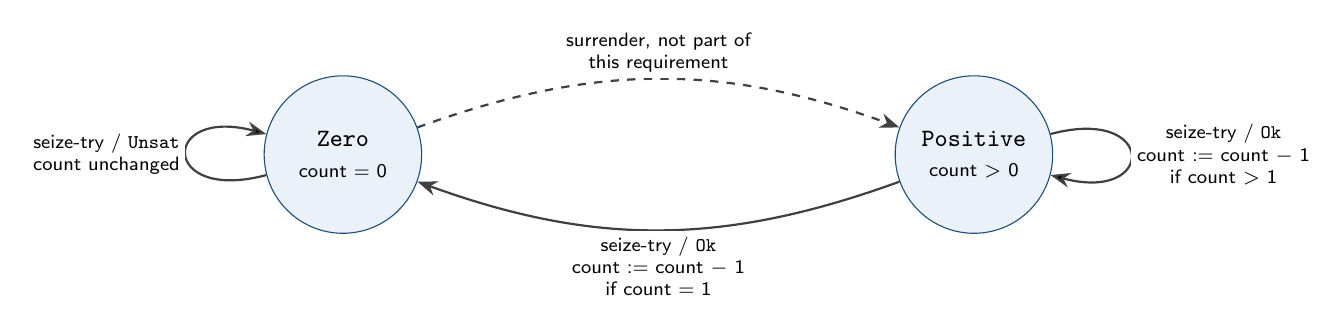
\begin{tikzpicture}[
    font=\small, node distance=60mm,
    st/.style={state, draw=ebblue, fill=boxfill, minimum size=20mm,
      align=center},
    edge/.style={-{Stealth[length=2.5mm]}, thick, draw=flow},
    lbl/.style={font=\scriptsize, align=center, fill=white, inner sep=2pt}]
  \node[st] (zero) {\texttt{Zero}\\\scriptsize count = 0};
  \node[st, right=of zero] (pos) {\texttt{Positive}\\\scriptsize count \textgreater{} 0};
  \draw[edge] (zero) edge[loop left, min distance=14mm] node[lbl, left]
    {seize-try / \texttt{Unsat}\\count unchanged} (zero);
  \draw[edge] (pos) edge[loop right, min distance=14mm] node[lbl, right]
    {seize-try / \texttt{Ok}\\count := count $-$ 1\\if count \textgreater{} 1} (pos);
  \draw[edge] (pos) to[bend left=20] node[lbl, below]
    {seize-try / \texttt{Ok}\\count := count $-$ 1\\if count = 1} (zero);
  \draw[edge, dashed] (zero) to[bend left=20] node[lbl, above]
    {surrender, not part of\\this requirement} (pos);
\end{tikzpicture}
\end{document}
